%% 
%% Copyright 2007, 2008, 2009 Elsevier Ltd
%% 
%% This file is part of the 'Elsarticle Bundle'.
%% ---------------------------------------------
%% 
%% It may be distributed under the conditions of the LaTeX Project Public
%% License, either version 1.2 of this license or (at your option) any
%% later version.  The latest version of this license is in
%%    http://www.latex-project.org/lppl.txt
%% and version 1.2 or later is part of all distributions of LaTeX
%% version 1999/12/01 or later.
%% 
%% The list of all files belonging to the 'Elsarticle Bundle' is
%% given in the file `manifest.txt'.
%% 
%% Template article for Elsevier's document class `elsarticle'
%% with harvard style bibliographic references
%% SP 2008/03/01

\documentclass[preprint,12pt,authoryear]{elsarticle}

%% Use the option review to obtain double line spacing
%% \documentclass[authoryear,preprint,review,12pt]{elsarticle}

%% Use the options 1p,twocolumn; 3p; 3p,twocolumn; 5p; or 5p,twocolumn
%% for a journal layout:
%% \documentclass[final,1p,times,authoryear]{elsarticle}
%% \documentclass[final,1p,times,twocolumn,authoryear]{elsarticle}
%% \documentclass[final,3p,times,authoryear]{elsarticle}
%% \documentclass[final,3p,times,twocolumn,authoryear]{elsarticle}
%% \documentclass[final,5p,times,authoryear]{elsarticle}
%% \documentclass[final,5p,times,twocolumn,authoryear]{elsarticle}

%% For including figures, graphicx.sty has been loaded in
%% elsarticle.cls. If you prefer to use the old commands
%% please give \usepackage{epsfig}

%% The amssymb package provides various useful mathematical symbols
\usepackage{amssymb}
\usepackage{amsmath}
\usepackage{color, soul}
\usepackage{url}
%% The amsthm package provides extended theorem environments
%% \usepackage{amsthm}

%% The lineno packages adds line numbers. Start line numbering with
%% \begin{linenumbers}, end it with \end{linenumbers}. Or switch it on
%% for the whole article with \linenumbers.
\usepackage{lineno}

%% Block of code for fixing corresponding author bug 
%% in elsarticle template... Don't really understand it
\makeatletter
\def\@author#1{\g@addto@macro\elsauthors{\normalsize%
    \def\baselinestretch{1}%
    \upshape\authorsep#1\unskip\textsuperscript{%
      \ifx\@fnmark\@empty\else\unskip\sep\@fnmark\let\sep=,\fi
      \ifx\@corref\@empty\else\unskip\sep\@corref\let\sep=,\fi
      }%
    \def\authorsep{\unskip,\space}%
    \global\let\@fnmark\@empty
    \global\let\@corref\@empty  %% Added
    \global\let\sep\@empty}%
    \@eadauthor={#1}
}
\makeatother
%% End block of weird code


%% Command for bold Greek symbols
\newcommand{\mitbf}[1]{\hbox{\mathversion{bold}$#1$}}

\journal{Earth and Planetary Science Letters}

\begin{document}

\begin{frontmatter}

%% Title, authors and addresses

%% use the tnoteref command within \title for footnotes;
%% use the tnotetext command for theassociated footnote;
%% use the fnref command within \author or \address for footnotes;
%% use the fntext command for theassociated footnote;
%% use the corref command within \author for corresponding author footnotes;
%% use the cortext command for theassociated footnote;
%% use the ead command for the email address,
%% and the form \ead[url] for the home page:
%% \title{Title\tnoteref{label1}}
%% \tnotetext[label1]{}
%% \author{Name\corref{cor1}\fnref{label2}}
%% \ead{email address}
%% \ead[url]{home page}
%% \fntext[label2]{}
%% \cortext[cor1]{}
%% \address{Address\fnref{label3}}
%% \fntext[label3]{}

\title{Bayesian inversion for paleomagnetic reconstruction and plate kinematics}

%% use optional labels to link authors explicitly to addresses:
%% \author[label1,label2]{}
%% \address[label1]{}
%% \address[label2]{}

\author{Ian Rose\corref{cor1}\fnref{ref1}}
\author{Bruce Buffett\fnref{ref1}}
\author{N.L. Swanson-Hysell\fnref{ref1}}

\fntext[ref1]{University of California, Berkeley}
\cortext[cor1]{Corresponding author, \url{ian.rose@berkeley.edu}}

\address{}

\begin{abstract}
%% Text of abstract

\end{abstract}

\begin{keyword}
%% keywords here, in the form: keyword \sep keyword

%% PACS codes here, in the form: \PACS code \sep code

%% MSC codes here, in the form: \MSC code \sep code
%% or \MSC[2008] code \sep code (2000 is the default)

\end{keyword}

\end{frontmatter}

\linenumbers

%% main text
\section{Introduction}
\label{sec:introduction}

\section{Interpretation of APW paths}
\label{sec:pep}

\subsection{Latitudinal drift}
\subsection{Running means and spline fits}
\subsection{Paleomagnetic Euler poles}
\citet{gordon1984paleomagnetic}

\section{Bayesian inversion}
\label{sec:bayesian_inversion}
\subsection{Bayes theorem}
\subsection{Distributions on a sphere}

\begin{figure*}
\includegraphics[width=0.9\textwidth]{figures/uniform.pdf}
\caption{Probability density for the Fisher distribution, as well as samples drawn from that distribution, plotted with an orthographic projection.}
\label{fig:uniform}
\end{figure*}

\subsubsection{Uniform distribution}
\begin{equation}
  \rho(\psi, \phi) = \frac{1}{4 \pi}
\end{equation}
\subsubsection{Fisher distribution}
\begin{equation}
  \begin{aligned}
  \rho(\psi, \phi) 
  &= \frac{1}{C_F} \exp \left( \kappa_F \hat{\mathbf{x}}^T \hat{\mitbf{\mu}} \right) \\
  &= \frac{1}{C_F} \exp \left( \kappa_F \cos \theta \right)
  \end{aligned}
\end{equation}
\begin{equation}
  C_F = \frac{\kappa_F}{4 \pi \sinh{\kappa}}
\end{equation}

\begin{figure*}
\includegraphics[width=0.9\textwidth]{figures/fisher.pdf}
\caption{Probability density for a uniform spherical distribution, as well as samples drawn from that distribution, plotted with an orthographic projection. The center of the distribution is at $30^\circ$N, $30^\circ$E, and the concentration parameter $\kappa=20$.}
\label{fig:fisher}
\end{figure*}

\subsubsection{Watson distribution}
\begin{equation}
  \begin{aligned}
  \rho(\psi, \phi) 
  &= \frac{1}{C_W} \exp \left( \kappa_W (\hat{\mathbf{x}}^T \hat{\mitbf{\mu}})^2 \right) \\
  &= \frac{1}{C_W} \exp \left( \kappa_W \cos^2 \theta \right)
  \end{aligned}
\end{equation}
\begin{equation}
  C_W = \left[ {}_1 F_1 \left( \frac{1}{2}, \frac{3}{2}, \kappa_W \right) \right]^{-1}
\end{equation}

\begin{figure*}
\includegraphics[width=0.9\textwidth]{figures/watson.pdf}
\caption{Probability density for the Watson girdle distribution, as well as samples drawn from that distribution, plotted with an Orthographic projection. The pole of symmetry is at $70^\circ$N, $90^\circ$E, and the concentration parameter $\kappa=-5$.}
\label{fig:watson}
\end{figure*}
\subsection{Markov chain Monte Carlo methods}

\section{Choice of priors}
\label{sec:priors}
\subsection{Euler poles}
\subsection{Ages}

\section{Model selection}
\label{sec:model_selection}

\section{Example inversions}
\label{sec:example_inversion}
\subsection{One stage pole}
\begin{figure*}
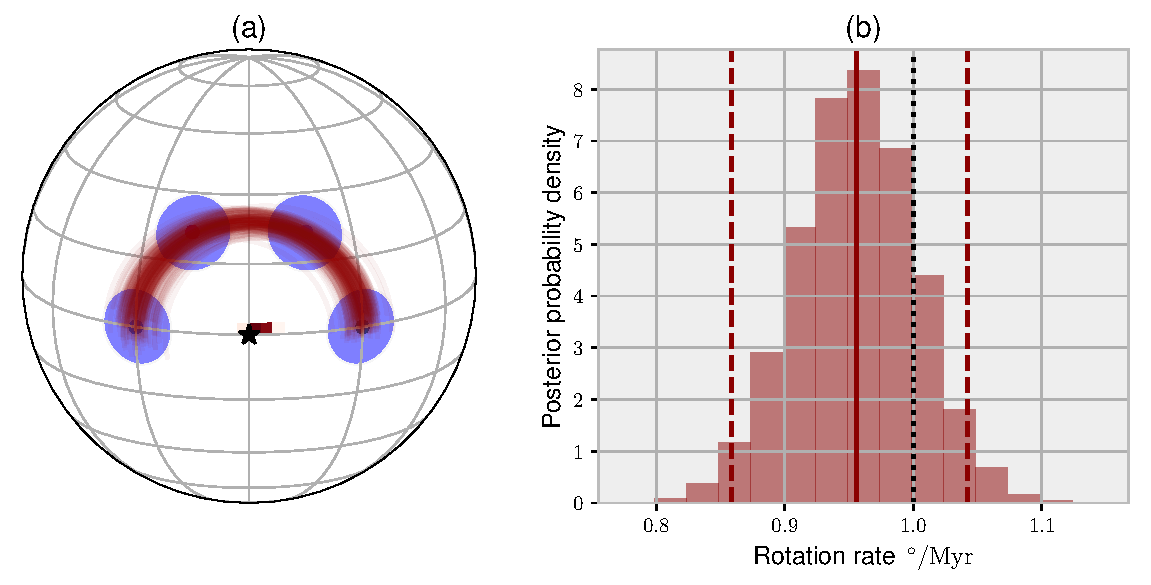
\includegraphics[width=0.9\textwidth]{figures/one_euler_pole.pdf}
\caption{Inversion for a single paleomagnetic Euler pole (PEP). (a) Four paleomagnetic poles are generated by a $180^\circ$ rotation about an Euler pole at $0^\circ$N, $0^\circ$E over 30 Myr, for a rotation rate of $6^\circ$/Myr. The red distribution is the probability density function recovered by MCMC inversion, and the red lines are a sampling of the synthetic APW paths generated by the inversion. (b) Posterior probability density for the rotation rate of the Euler pole recovered by the inversion. The peak of the distribution slightly underestimates the true value of $6^\circ$/Myr, and the great majority of the probability lies between $4^\circ-7^\circ$/Myr. }
\label{fig:one_euler_pole}
\end{figure*}

\subsection{Two stage poles}
\begin{figure*}
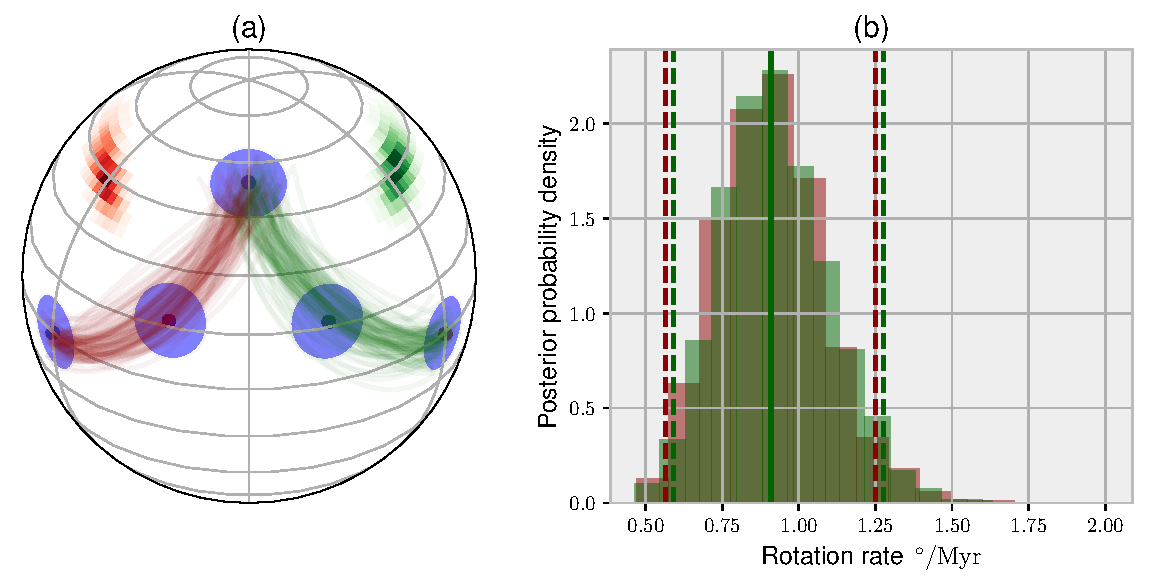
\includegraphics[width=0.9\textwidth]{figures/two_euler_poles.pdf}
\caption{Inversion for two successive paleomagnetic Euler poles. (a) Five paleomagnetic poles are generated, beginning with a pole at $0^\circ$N, $60^\circ$W. The first Euler pole is located at $41^\circ$N, $60^\circ$W, and rotates at $6.5^\circ$/Myr for 20 Myr. The second Euler pole is located at $41^\circ$N, $60^\circ$W, and rotates at the same speed and for the same duration. The red and green distributions show the location of the first and second Euler poles (respectively) recovered by the MCMC inversion. The the red and green lines are a sampling of the synthetic APW paths generated by the inversion. (b) Posterior probability density for the rotation rates of the Euler poles recovered by the inversion.}
\label{fig:two_euler_poles}
\end{figure*}
\subsection{Incorporating age uncertainty}

\section{Application to Cenozoic Australian APW path}
\clearpage
\begin{figure*}
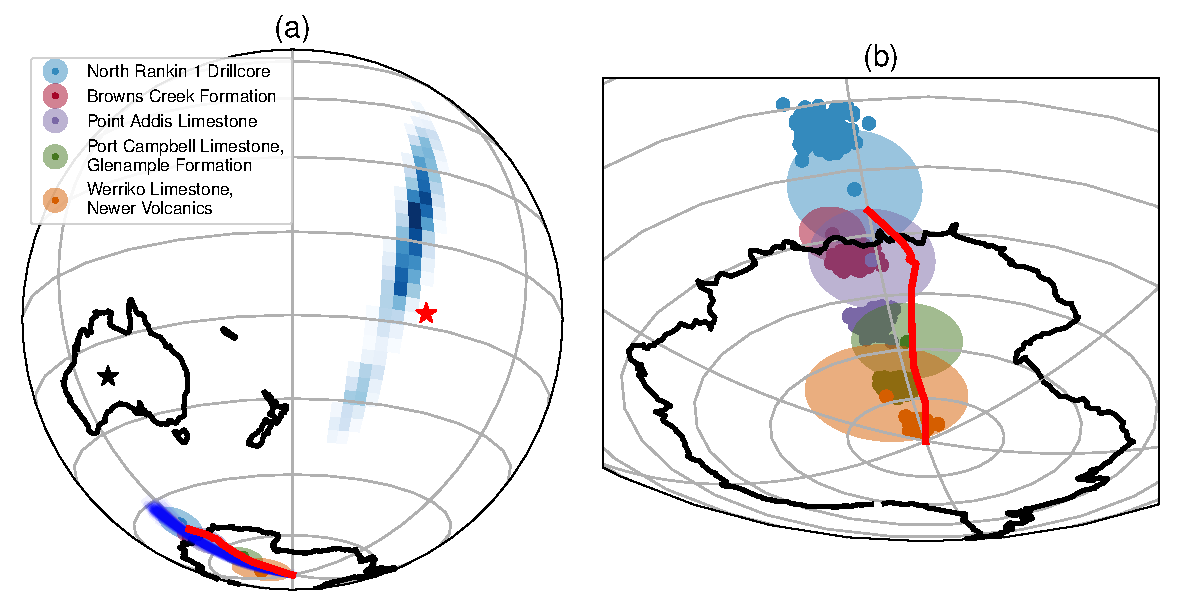
\includegraphics[width=0.9\textwidth]{figures/australia/australia_paths_1.pdf}
\caption{}
\label{fig:australia_paths_1}
\end{figure*}
\begin{figure*}
\includegraphics[width=0.9\textwidth]{figures/australia/australia_ages_1.pdf}
\caption{}
\label{fig:australia_ages_1}
\end{figure*}
\begin{figure*}
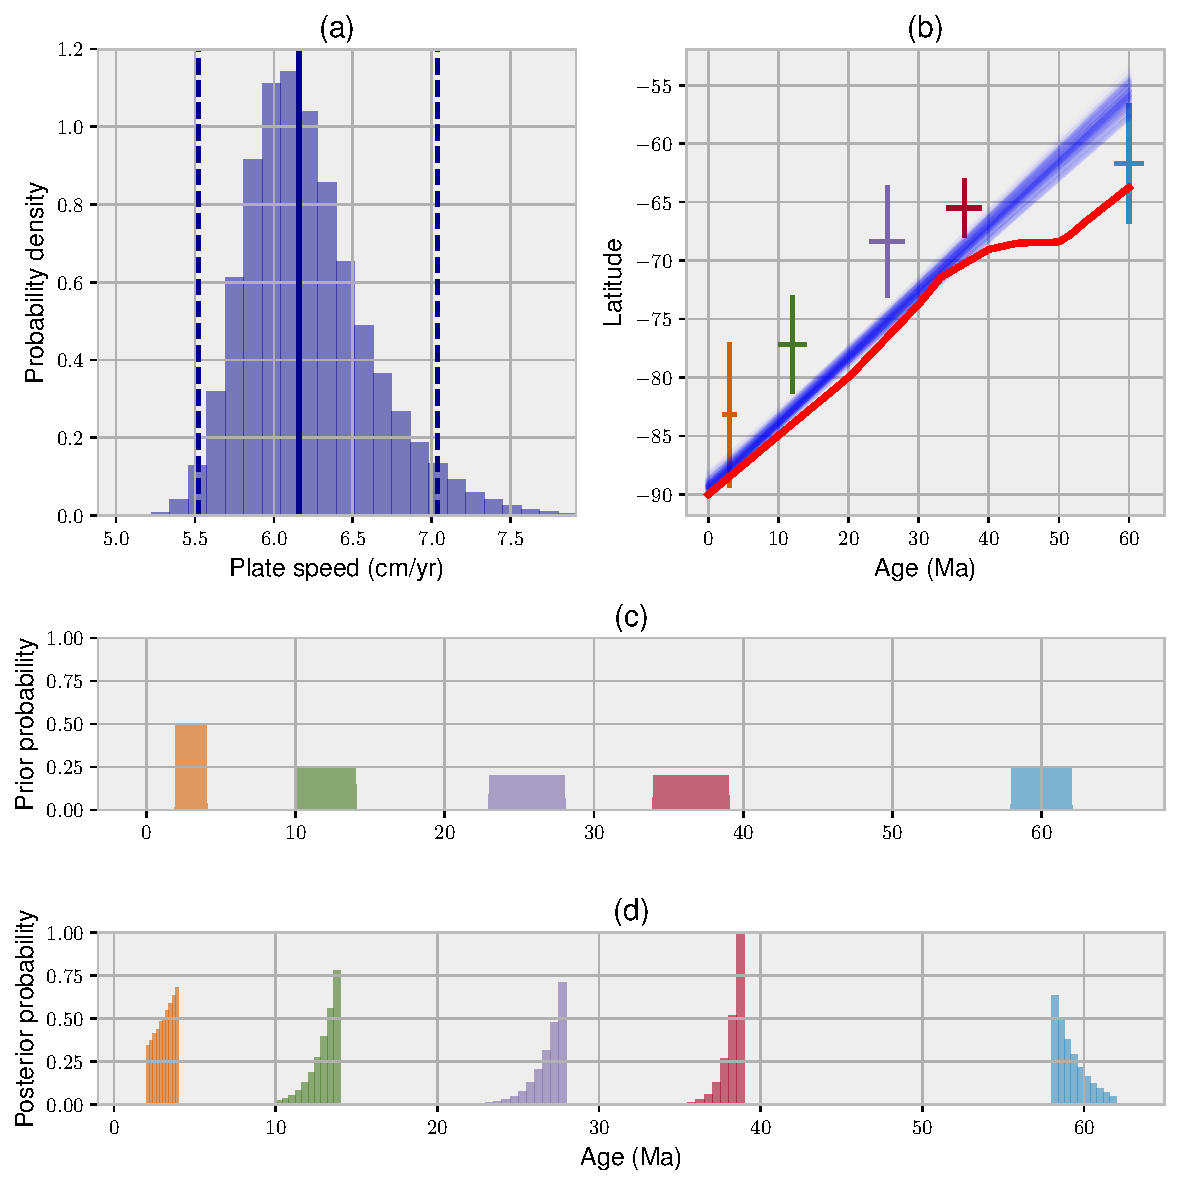
\includegraphics[width=0.9\textwidth]{figures/australia/australia_speeds_1.pdf}
\caption{}
\label{fig:australia_speeds_1}
\end{figure*}
\begin{figure*}
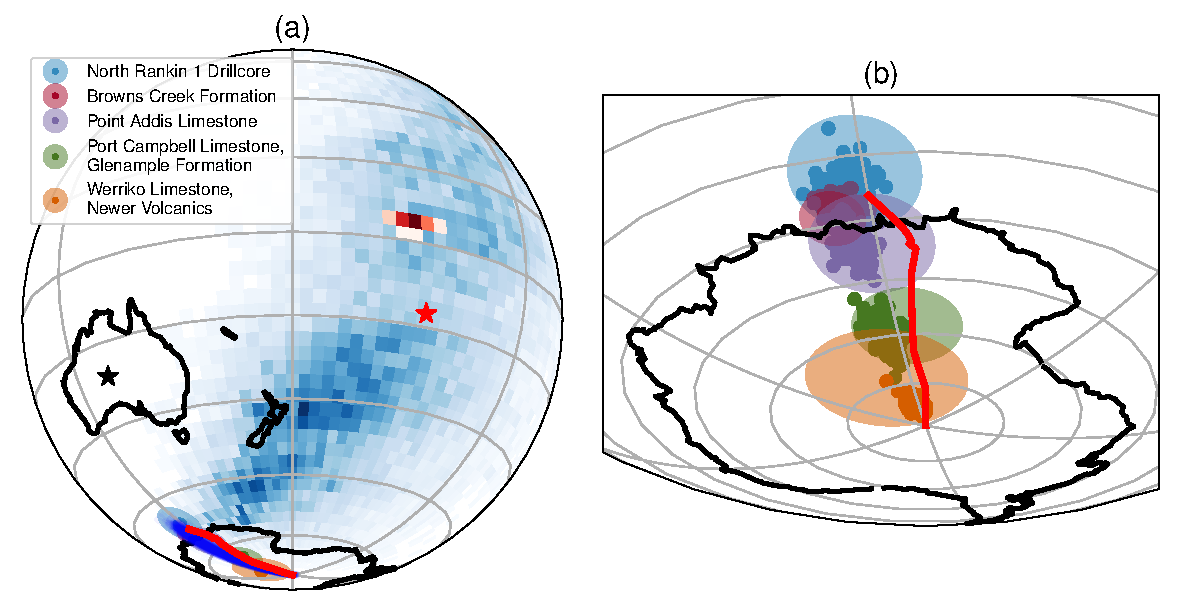
\includegraphics[width=0.9\textwidth]{figures/australia/australia_paths_2.pdf}
\caption{}
\label{fig:australia_paths_2}
\end{figure*}
\begin{figure*}
\includegraphics[width=0.9\textwidth]{figures/australia/australia_ages_2.pdf}
\caption{}
\label{fig:australia_ages_2}
\end{figure*}
\begin{figure*}
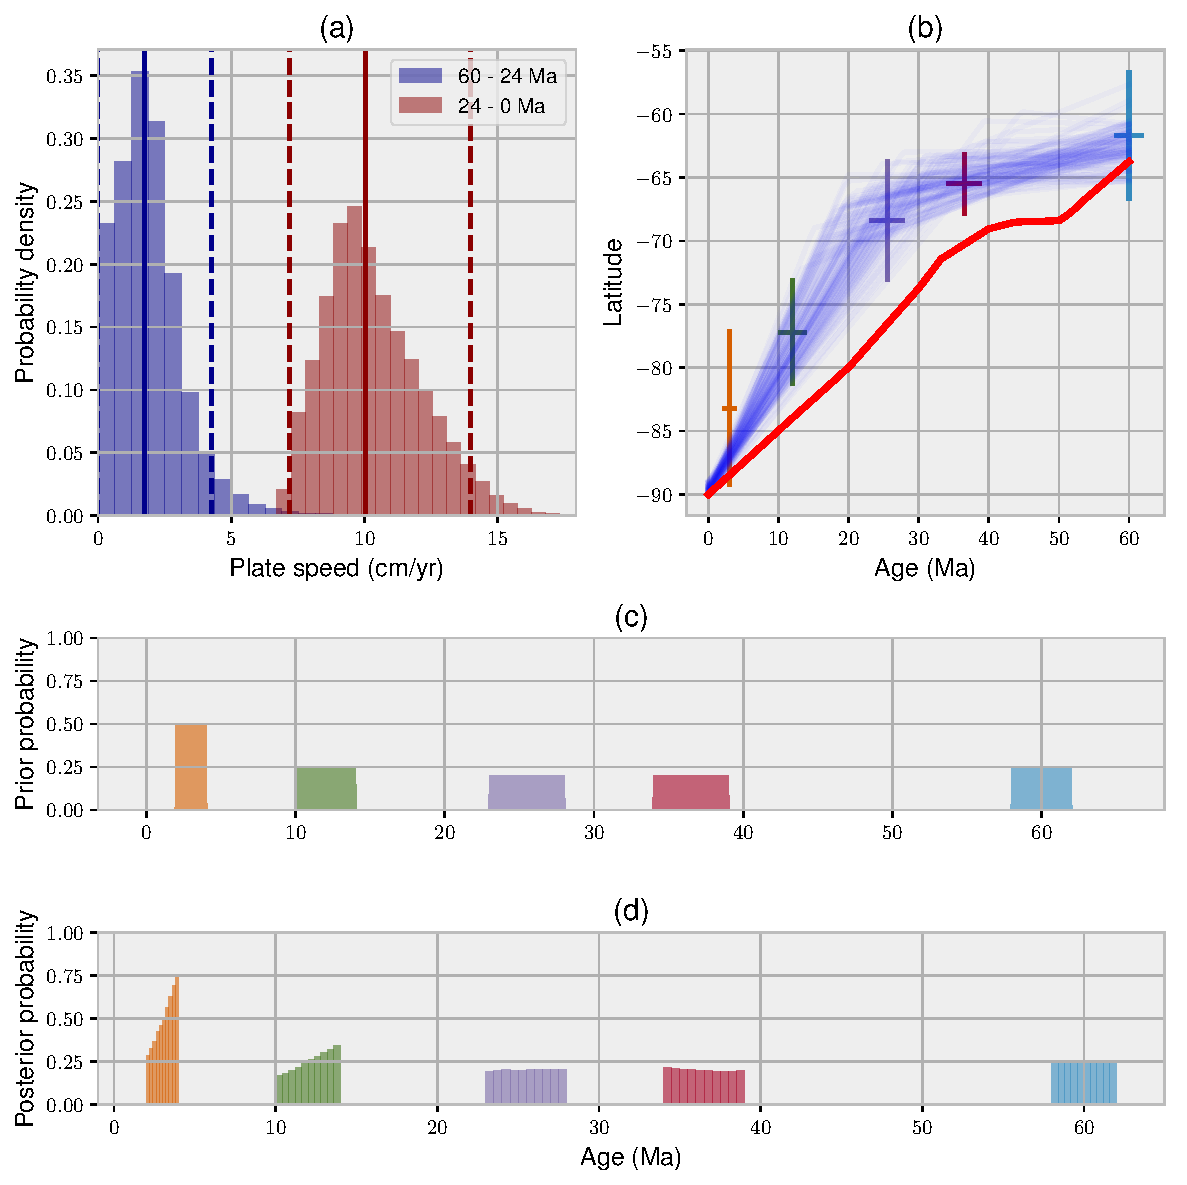
\includegraphics[width=0.9\textwidth]{figures/australia/australia_speeds_2.pdf}
\caption{}
\label{fig:australia_speeds_2}
\end{figure*}


\section{Application to the Keweenawan province}
\label{sec:keweenawan}
\subsection{Geologic context}
\citet{swanson2009no}
\subsection{Inversion for paleomagnetic Euler poles}
\clearpage
\begin{figure*}
\includegraphics[width=0.9\textwidth]{figures/keweenawan/keweenawan_paths_1.pdf}
\caption{}
\label{fig:keweenawan_paths_1}
\end{figure*}
\begin{figure*}
\includegraphics[width=0.9\textwidth]{figures/keweenawan/keweenawan_ages_1.pdf}
\caption{}
\label{fig:keweenawan_ages_1}
\end{figure*}
\begin{figure*}
\includegraphics[width=0.9\textwidth]{figures/keweenawan/keweenawan_speeds_1.pdf}
\caption{}
\label{fig:keweenawan_speeds_1}
\end{figure*}
\begin{figure*}
\includegraphics[width=0.9\textwidth]{figures/keweenawan/keweenawan_paths_2.pdf}
\caption{}
\label{fig:keweenawan_paths_2}
\end{figure*}
\begin{figure*}
\includegraphics[width=0.9\textwidth]{figures/keweenawan/keweenawan_ages_2.pdf}
\caption{}
\label{fig:keweenawan_ages_2}
\end{figure*}
\begin{figure*}
\includegraphics[width=0.9\textwidth]{figures/keweenawan/keweenawan_speeds_2.pdf}
\caption{}
\label{fig:keweenawan_speeds_2}
\end{figure*}
\begin{figure*}
\includegraphics[width=0.9\textwidth]{figures/keweenawan/keweenawan_paths_3.pdf}
\caption{}
\label{fig:keweenawan_paths_3}
\end{figure*}
\begin{figure*}
\includegraphics[width=0.9\textwidth]{figures/keweenawan/keweenawan_ages_3.pdf}
\caption{}
\label{fig:keweenawan_ages_3}
\end{figure*}
\begin{figure*}
\includegraphics[width=0.9\textwidth]{figures/keweenawan/keweenawan_speeds_3.pdf}
\caption{}
\label{fig:keweenawan_speeds_3}
\end{figure*}
\subsection{Plate speeds for Mesoproterozoic Laurentia}

\section{Conclusions}
\label{sec:conclusions}



%% The Appendices part is started with the command \appendix;
%% appendix sections are then done as normal sections
%% \appendix

%% \section{}
%% \label{}

%% If you have bibdatabase file and want bibtex to generate the
%% bibitems, please use
%%
\bibliographystyle{elsarticle-harv} 
\bibliography{bayesian_plate_reconstruction}

%% else use the following coding to input the bibitems directly in the
%% TeX file.

\end{document}

\endinput
%%
%% End of file `elsarticle-template-harv.tex'.
